%
% $RCSfile: new_systematics.tex,v $
%
% Copyright (c) 2004. Christian Heller. All rights reserved.
%
% No copying, altering, distribution or any other actions concerning this
% document, except after explicit permission by the author!
% At some later point in time, this document is planned to be put under
% the GNU FDL license. For now, _everything_ is _restricted_ by the author.
%
% http://www.cybop.net
% - Cybernetics Oriented Programming -
%
% http://www.resmedicinae.org
% - Information in Medicine -
%
% @author Christian Heller <christian.heller@tuxtax.de>
%

\section{New Systematics}
\label{new_systematics_heading}

Section \ref{pattern_heading} used traditional proposals \cite{buschmann,gamma1995}
to systematize patterns and divided them according to the first categorization
level shown in figure \ref{pattern_figure}. The following sections will work out
a new systematics, to classify patterns.

%
% $RCSfile: human_thinking.tex,v $
%
% Copyright (c) 2004. Christian Heller. All rights reserved.
%
% No copying, altering, distribution or any other actions concerning this
% document, except after explicit permission by the author!
% At some later point in time, this document is planned to be put under
% the GNU FDL license. For now, _everything_ is _restricted_ by the author.
%
% http://www.cybop.net
% - Cybernetics Oriented Programming -
%
% http://www.resmedicinae.org
% - Information in Medicine -
%
% @author Christian Heller <christian.heller@tuxtax.de>
%

\subsection{Human Thinking}
\label{human_thinking_heading}

The new classification is based on the idea of categorizing software patterns
after the principles of \emph{Human Thinking}, that is concepts of the logical
\emph{Mind}, as opposed to \emph{Artificial Neural Networks} (ANN) that want to
imitate the functioning of the physical \emph{Brain}.

The corresponding concepts were first introduced in \cite{heller2004}. After an
investigation of the fundamentals of human thinking, that is how human beings
understand their surrounding real world by abstracting it in \emph{Models}, that
paper concludes that there were three basic activities of abstraction:

\begin{enumerate}
    \item Discrimination
    \item Categorization
    \item Composition
\end{enumerate}

By discriminating their environment, humans are able to share it into discrete
\emph{Items}. Items with similar properties can be classified into a common super
\emph{Category}. Any abstract model of the universe is just an illusion, being
made up of yet smaller models, and nobody knows where this hierarchy really stops,
towards microcosm as well as towards macrocosm. Therefore, the third and last
kind of abstraction, namely composition, lets humans perceive the items in their
environment as \emph{Compound} of smaller items.

\begin{figure}[ht]
    \begin{center}
        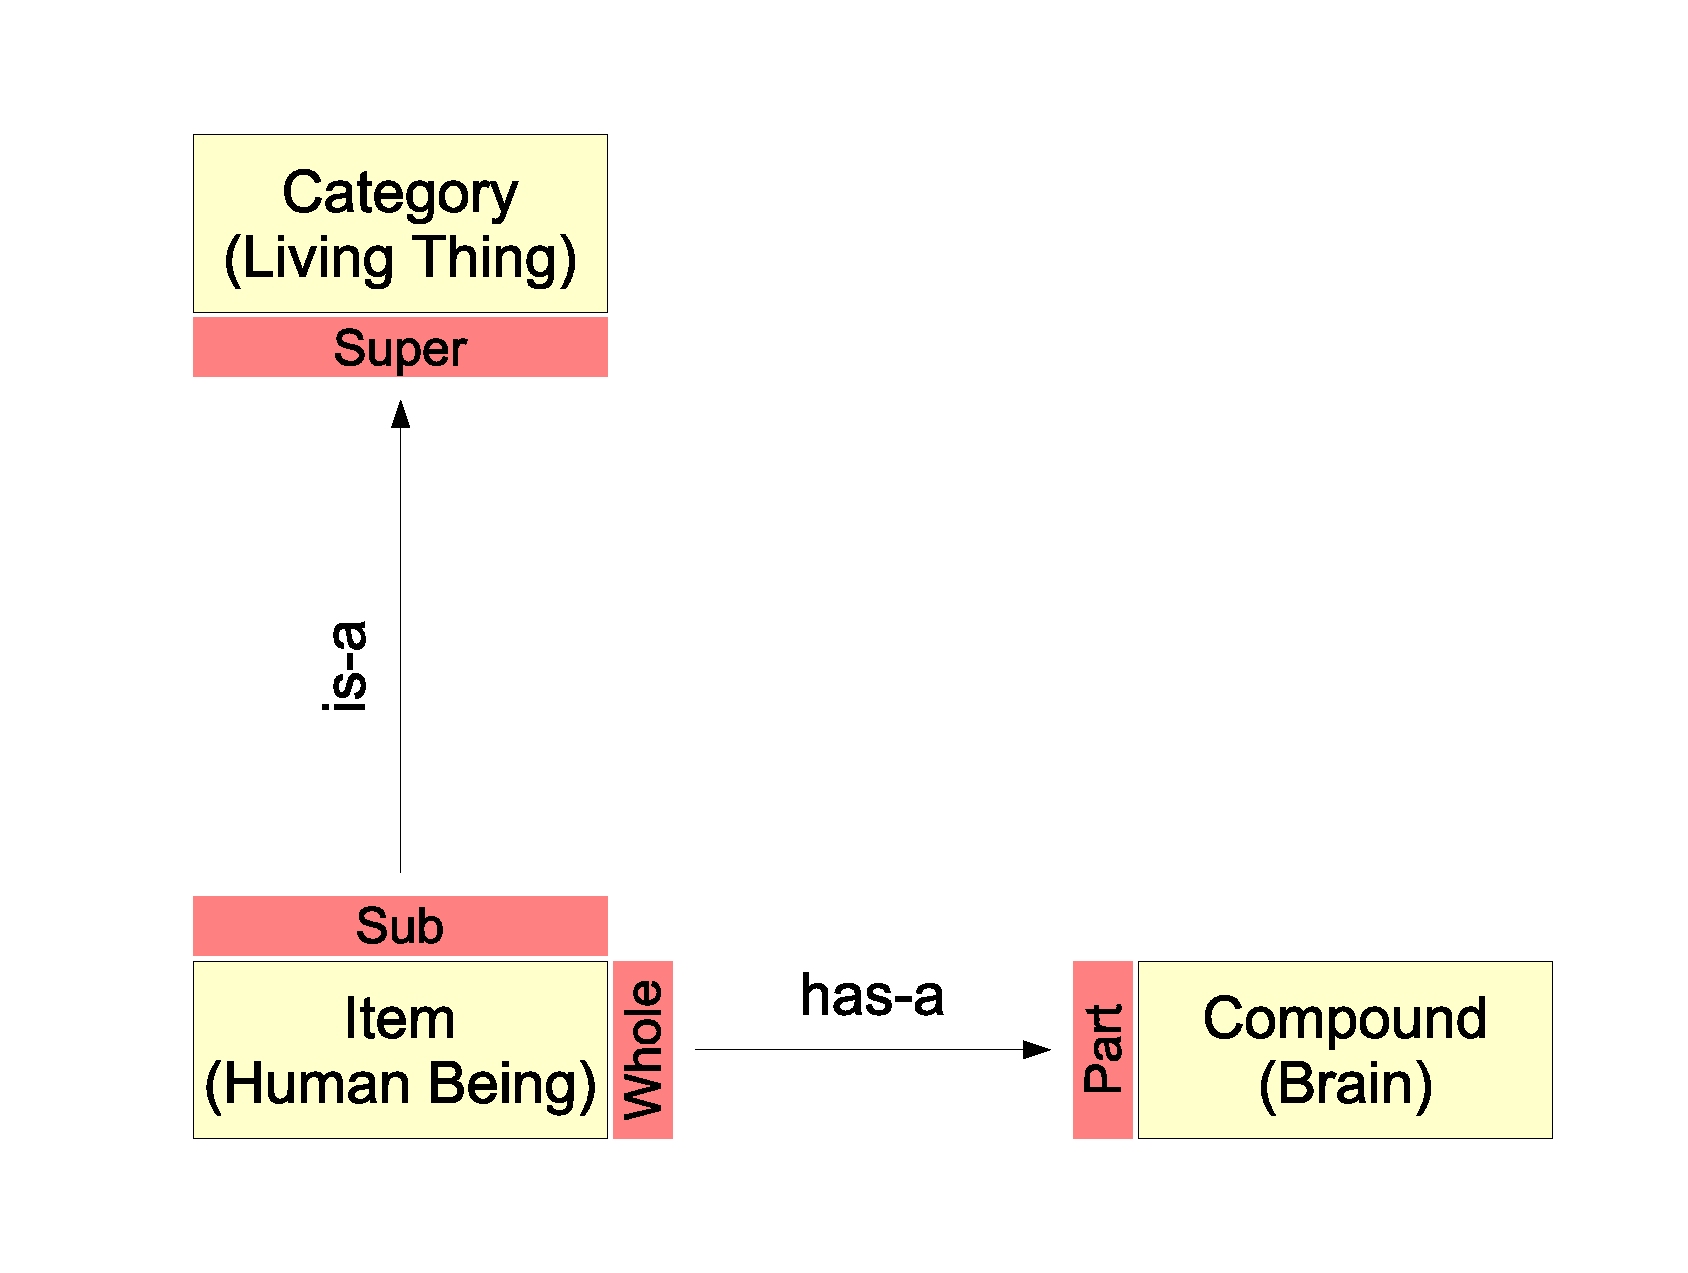
\includegraphics[scale=0.3]{vector/abstraction.eps}
        \caption{Abstractions of Human Thinking \cite{heller2004}}
        \label{abstraction_figure}
    \end{center}
\end{figure}

The latter two activities of abstraction -- categorization and composition --
are based on special \emph{Associations} (figure \ref{abstraction_figure}),
between a \emph{Super-} and a \emph{Sub} model and between a \emph{Whole-} and
a \emph{Part} model, respectively.

%
% $RCSfile: categories.tex,v $
%
% Copyright (c) 2004. Christian Heller. All rights reserved.
%
% No copying, altering, distribution or any other actions concerning this
% document, except after explicit permission by the author!
% At some later point in time, this document is planned to be put under
% the GNU FDL license. For now, _everything_ is _restricted_ by the author.
%
% http://www.cybop.net
% - Cybernetics Oriented Programming -
%
% http://www.resmedicinae.org
% - Information in Medicine -
%
% @author Christian Heller <christian.heller@tuxtax.de>
%

\subsection{Categories}
\label{categories_heading}

Most patterns heavily rely on associations, too. This paper therefore suggests to:

\begin{center}
    \textbf{Take the Kind of Association as Criterion\\
    to sort patterns in a completely new way.}
\end{center}

The opposite table shows a systematics of the new pattern categories with their
equivalents in human thinking, some representative example patterns and a
recommendation for their usage in software engineering. Patterns matching into
more than one category are placed after the priority: \emph{Recursion} over
\emph{Polymorphism}.

\begin{table}[ht]
    \begin{center}
        \begin{tabular}{| p{22mm} | p{20mm} | p{23mm} | p{10mm} |}
            \hline
            \textbf{Category} & \textbf{Equivalent} & \textbf{Representative} & \textbf{Advice}\\
            \hline
            Itemization & Discrimination & Command, Data Transfer Object, State, Memento, Envelope-Letter, Prototype & :-)\\
            \hline
            1:1 Association & Composition & Delegator, Object Adapter, Proxy (Surrogat, Client-/Server Stub), Wrapper, Handle-Body, Bridge & :-)\\
            \hline
            1:n Association & Composition & Whole-Part, View Handler, Broker (Mediator), Master-Slave, Command Processor, Counted Pointer, Chain of Responsibility & :-)\\
            \hline
            Recursion & Composition & Composite, Interpreter, Decorator, Linked Wrapper & :-)\\
            \hline
            Bidirectionalism & -- & Observer (Callback, Publisher-Subscriber), Forwarder-Receiver, Chain of Responsibility, Visitor, Reflection & :-(\\
            \hline
            Polymorphism & Categorization & Template Method, Builder, Factory Method, Class Adapter, Abstract Factory (Kit), Strategy (Validator, Policy), Iterator (Cursor) & :-$\mid$\\
            \hline
            Grouping & Categorization & Layers, Domain Model, MVC & :-)\\
            \hline
            Global Access & -- & Singleton, Flyweight, Registry, Manager & :-(\\
            \hline
        \end{tabular}
%        \caption{Pattern Systematics}
        \label{pattern_systematics_table}
    \end{center}
\end{table}

%
% $RCSfile: recommendation.tex,v $
%
% Copyright (c) 2004. Christian Heller. All rights reserved.
%
% No copying, altering, distribution or any other actions concerning this
% document, except after explicit permission by the author!
% At some later point in time, this document is planned to be put under
% the GNU FDL license. For now, _everything_ is _restricted_ by the author.
%
% http://www.cybop.net
% - Cybernetics Oriented Programming -
%
% http://www.resmedicinae.org
% - Information in Medicine -
%
% @author Christian Heller <christian.heller@tuxtax.de>
%

\subsection{Recommendation}
\label{recommendation_heading}

The first category \emph{Itemization} (objectification) is the base of any
modelling activity and clearly necessary.

The next three categories \emph{1:1 Association}, \emph{1:n Association} and
\emph{Recursion} are special kinds of associations that rely exclusively on
\emph{unidirectional} relations and result in a clean architecture which is why
their usage is strongly recommended.

\emph{Bidirectionalism}, on the other hand, is an \emph{ill} variant of the three
aforementioned categories and should be avoided wherever possible. Patterns in
this category are one reason for endless loops and unpredictable behaviour since
it becomes very difficult to trace the effects that changes in one place of a
system have on others (section \ref{bidirectional_dependency_heading}).

\emph{Polymorphism} is a good thing. It relies on categorization and due to
inheritance can avoid a tremendous amount of otherwise redundant source code.
However, it also makes understanding a system more difficult, since the whole
architecture must be understood before being able to manipulate code correctly.
Unwanted source code changes caused by inheritance dependencies are often
described with the term \emph{Fragile Base Class Problem}
\cite[section \emph{Layers}]{buschmann}. They are just the opposite of what
inheritance was actually intended to be for: \emph{Reusability}
\cite[Vorwort]{gruhn}.

\emph{Grouping} models is essential to keep overview in a complex software
system. A very promising technology to support this are \emph{Ontologies}
\cite{hellerkunze}. A lot of thought-work has to go into them but if they are
well thought-out, they are clearly recommended.

The habit of globally accessing models is banned since OOP became popular.
However, it is not banned completely. Patterns like \emph{Singleton}
encapsulate and bundle global access but they still permit it. They disregard
any dependencies and relations in a system, such are a security risk and reason
for untraceable data changes. This paper sees the whole category of
\emph{Global Access} as potentially dangerous and can \emph{not} recommend its
patterns.

